\chapter{Methodology}

This chapter describe how a binary vocabulary test was designed based on the points highlighted in the literature review. When language-specific aspects of the methodology are mentioned, such as the sourcing of the types from an online Breton dictionary, it is understood that an analogue method can or has been used for a test in another language. 

\section{Sourcing the Keys}
One thing to understand about vocabulary recognition tests is that the they don't test words knowledge per se, because they dismiss the meaning of the words. As long as the string of character is associated with a dictionary entry, what one calls a word type, the item is real, and is expected to be recognised. In Breton, the word \textit{brec'h} means arm (the part of the body) like in Welsh \textit{braich}, but also (small) pox, like in Welsh \textit{brech}. Those are two distinct words and have always been. But when testing the type recognition skills, most test taker will most likely think ``arm'' and completely ignore the ``smallpox'' meaning, the knowledge of which would mean a higher vocabulary knowledge. It is even expectable that many would think that the word \textit{brec'hadur}, vaccine, is related to the meaning ``arm'', because they were inoculated vaccine in their arms and could not think of other etymologies. However, when facing the type \textit{brec'h-vihan}, ``small-pox'', what would these people think? Most likely something around this line: ``little-arm? in one word? which is the big-arm? this does not make any sense, it is not a real word''!. Only the people aware of the second meaning of the word \textit{brec'h} would recognize \textit{brec'h-vihan}.

This little example shows how how the types differs from words proper, and how their rating is expected to be levelled down to their simplest interpretation, although lesser known meaning can style be expected to be found in derived, more advanced terms.

For the Breton vocabulary test, all the entries of the Breton diachronic dictionary \href{https://devri.bzh/}{Devri} were fetched, and rules where designed to remove proper nouns and affixes. Since the monolingual dictionary \href{https://niverel.brezhoneg.bzh/br/meurgorf/}{Meurgorf} classifies its entries in one of three categories: frequent, common and rare, it was possible to organise the items in four categories, the three previous ones, and the items that were in Devri but not in Meurgorf. The distribution of the items is shown in~\ref{tab:breton-types}. The reasons why so many words seems to be absent in Devri, is that Meurgorf entries contain many proper nouns and affixes, as well as neologisms built with common affixes. The total number of available keys for the test was 62 169, half of which were given a rough difficulty rating between 1 and 3. The entries from Devri not found in Meurgorf were added the the category of the rare types.

\begin{table}[htbp]
    \centering
    \begin{tabular}{l|r|r|r}
        \textbf{Category} & \textbf{in Meurgorf} & \textbf{also in Devri} & \textbf{only in Devri} \\
        \hline
        Frequent & 1 108 & 946 & – \\
        Common & 47 740 & 26 197 & – \\
        Rare & 6 867 & 4 868 & – \\
        Total & 55 715 & 32 011 & 30 158 \\
    \end{tabular}
    \caption{Categories of word types extracted from Devri (filtered) and Meurgorf}
    \label{tab:breton-types}
\end{table}

Obviously these categories are not perfect, but they are still a precious help to the difficult questions of calibration. Other methods of sourcing types and different ranges of frequencies for other languages could include fetching the entries from dictionaries of different sizes. The entries present in the smaller dictionaries would be understood to be the most useful and frequent. The section on the rating initialization shows how these initial ratings are used. The code for these steps can be found on GitHub\footnote{For the sourcing of Devri's entries and their filtering, see \href{https://github.com/Oktogazh/sudogen/blob/master/1\%20Introduction.ipynb}{this Jupyter notebook}, for the the range of frequencies, see \href{https://github.com/Oktogazh/sudogen/blob/master/locales/br/5\%20Initialization.ipynb}{this other Jupyter notebook}}.

\section{Generating the Distractors}
    \abbrv{LSTM}{Long Short-Term Memory}
    \abbrv{RNN}{Recurrent Neural Network}
    \subsection{Training the Model}
For a study of the scale of this project, manually crafting the non-words is not an option. Different methods of computationally generate pseudo-words have been developed over the years, most of them chaining n-grams taken from a training dataset of various sizes \parencite{new_unipseudo_2023, keuleers_wuggy_2010}. However, since some languages are known to exhibit features of phonotactic long distance relationships, such as vowel harmony in Turkic languages, n-gram-based models were deemed non-optimal to generate unlikely pseudo-words. For this reason, the use of Long Short-Term Memory (LSTM) was privileged \parencite{hochreiter_long_1997}. The design will be straight-forward for people familiar with Recurrent Neural Network (RNN), but some optimization technics were developed to increase the speed of training. Since the words in the training dataset (the keys from the previous section) are of various lengths, no the batches are of length 1, which means that no parallelization was possible during training. To circumvent this problem, the words were concatenated in a hundred longer strings, with a new line character used as the special token, to start a sequence of words, to separate each word and to end each sequence, thus making these sequences both compact and human readable. 15 such sequences were kept for validation and 85 for training proper. Around 10 embedding dimensions (to represent the characters) and 180 hidden dimensions (to memorize the patterns) in the one LSTM cell were more than sufficient to train an "orthographic" language model able to generate good quality pseudo-words. Between 10 and 20 epochs are enough to obtain a low cross-entropy of below 1.8, and thank to the batching technique mentioned above, the training barely took around 10 to 12 second per epoch. Note however that a low cross-entropy was not systematically obtained, even with the same hyper-parameters. This is where another optimisation technique comes into play, a sensible effect on the loss function progression by to reshuffling the words in a different order and remake different sequences of around 620 word types. In a way, this was "generating more training data" where the only common point between the previous sequences and the new was the internal structure of the words, and the relationship between the words would not be taken into account by the LSTM hidden vector. This effectively swapped some words from the validating to the training set, but as the training dataset's loss function was consistently lower for all the trainings, thus showing no sign of overfitting even with large numbers of epoch, this was deemed not to be a problem.

    \subsection{Generation}
Once the character-based language model trained with a satisfying cross-entropy, it is ready to generate new words. Dividing the probability of the next token by an increasing temperature value increases the entropy of the softmax function distribution (last layer of the network) and thus tends to equalize the chance of the next token selected. It was found that a temperature of 0.7 was the sweet spot for a good balance between diversity and correctness of the characters generation. This sweet spot was found by looking at the proportion of words starting by the letter z, in Breton 1:2000 types start by a z. Obviously, different languages, especially languages with other alphabets would need another temperature.

As the goal for the network is to reproduce the training data with the biggest fidelity as possible, it will try to generated real words. The real words have to be filtered out, which was done in two different ways. Every time a new word was generated, when a new line character is generated, a new word is generated, the string is then compared with the available types in the training dataset, if it is not in the training dataset, the word is checked against a Hunspell spelling dictionary, and only if the spelling is not recognised, the word is added to a set generated pseudowords, with a high degree of confidence that the word is meaningless. The code for the generation of the pseudo-words is available on GitHub\footnote{See this \href{https://github.com/Oktogazh/sudogen/blob/master/2\%20Training.ipynb}{Jupyter notebook} for details}. This method was used to generate an equally large number of pseudo-words as real words, which was later used for statistical comparision of the two sets of strings.

\begin{figure}[htbp]
    \centering
    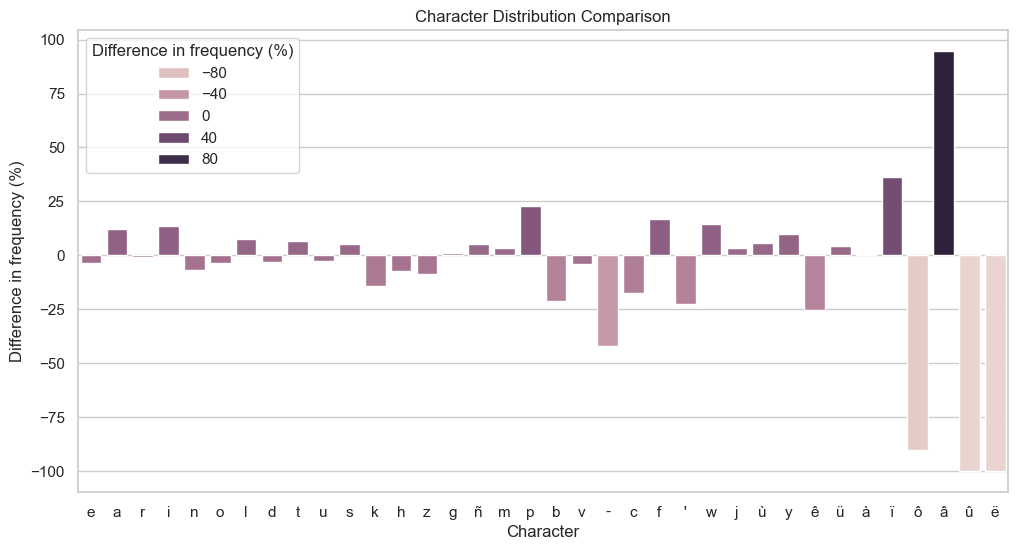
\includegraphics[width=0.8\textwidth]{figures/chars.png}
    \caption{Distribution of characters (pseudo-words / real words)}
\end{figure}\label{fig:chars}

As one thing that could give away a pseudo-word is the disproportion of some characters in the words, the Figure~\ref{fig:chars} is used to inspect the distribution of characters throughout the sets of words and pseudo-words. If the value for a given letter is positive, it means that a character is over-represented in the pseudo-words set, and the reverse if the value goes negative. The characters are ordered by frequency, \textit{e} being the most common character and \textit{ë} the rarest in Breton (found only once in the real words, and never in the pseudo words, hence the 100\% difference). Overall, the distribution of the character in the generated pseudo-words seems coherent with that of the real words.

\begin{figure}[htbp]
    \centering
    \begin{minipage}{0.45\textwidth}
        \centering
        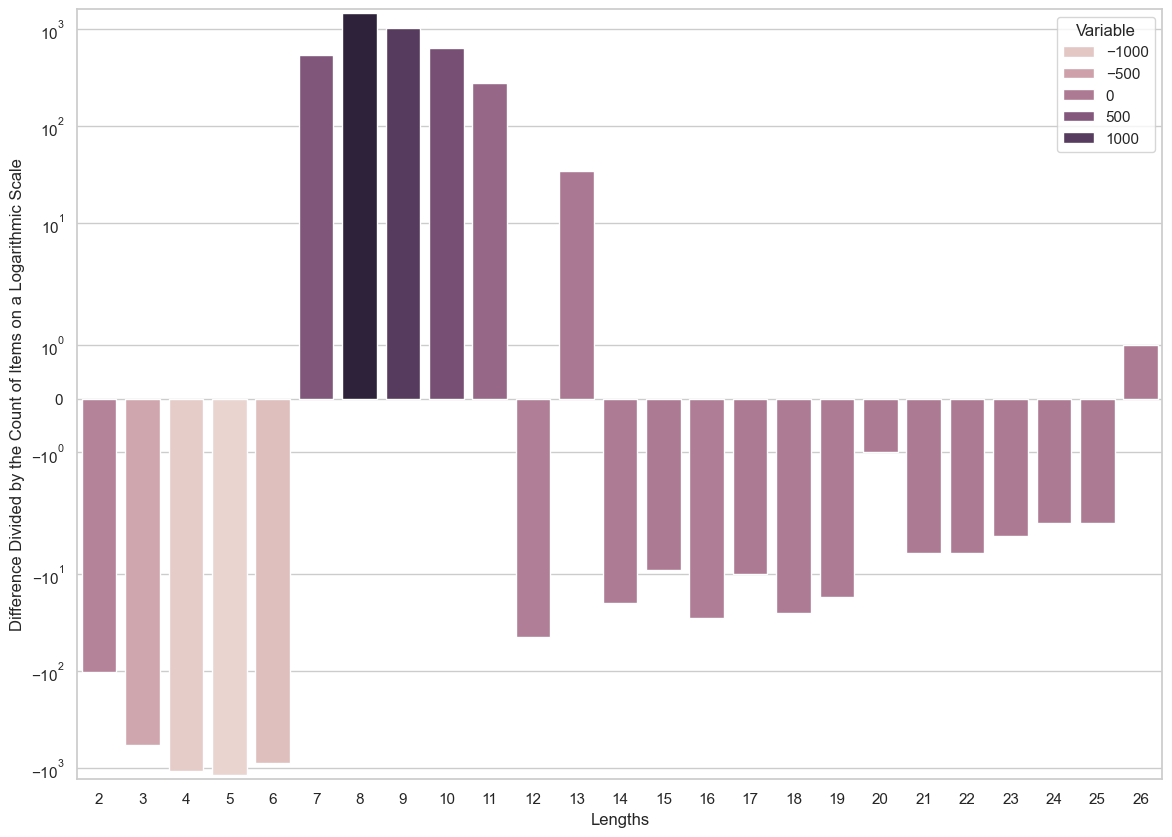
\includegraphics[width=0.8\textwidth]{figures/lengths.png}
        \caption{The difference between the count of pseudo-words over real words on a logarithmic scale for a given length.}\label{fig:lengths}
    \end{minipage}
    \hfill
    \begin{minipage}{0.45\textwidth}
        \centering
        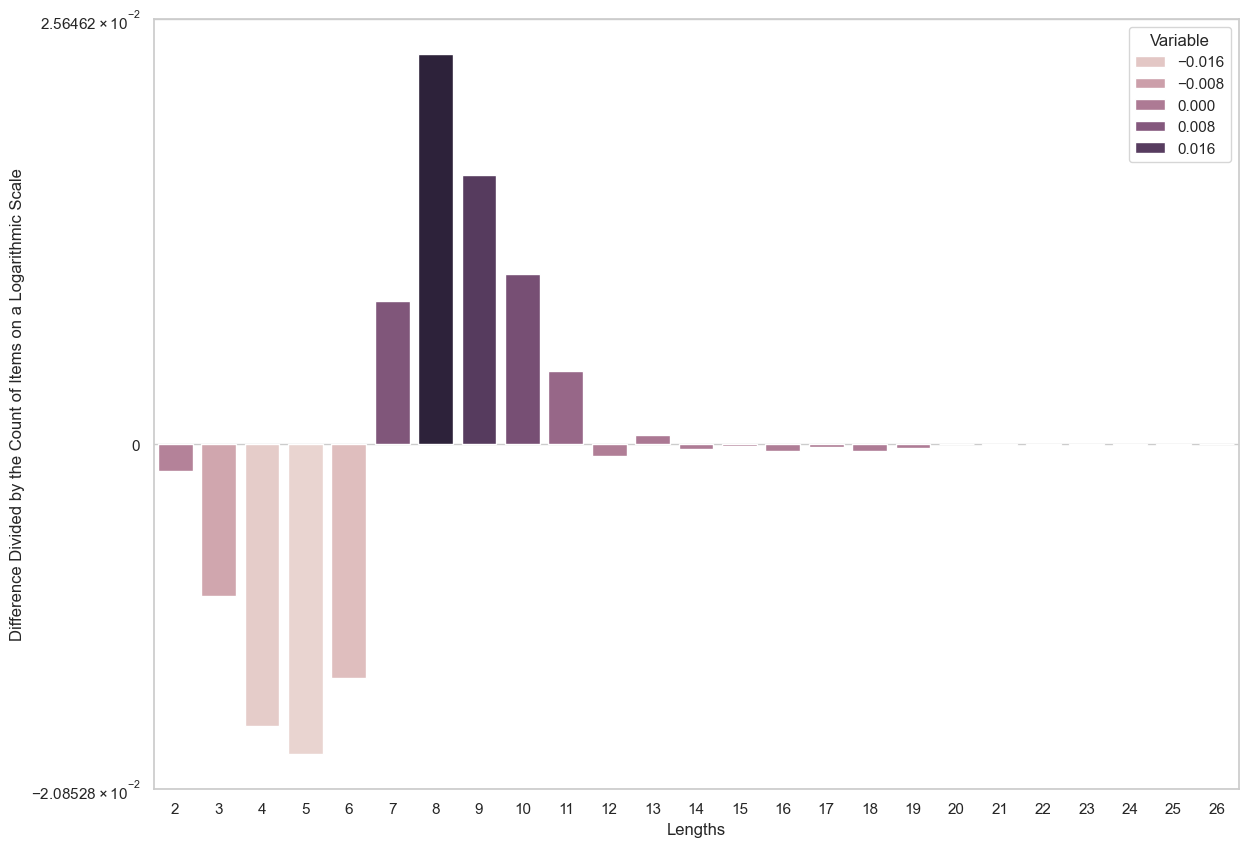
\includegraphics[width=0.8\textwidth]{figures/lengths_divided.png}
        \caption{The same difference as in~\ref{fig:lengths} divided by the total number of items to bring the differences in the context of a test session.}\label{fig:lengths_div}
    \end{minipage}
\end{figure}



The figures \ref{fig:lengths} and \ref{fig:lengths_div} are of particular interest. As the length differences could also give away clues to the test takers on whether a word is real or not. One can see that the network did not produce as many short pseudo-words as expected, where items of a length between 7 and 11 are over-represented to some degrees. This may be due to the fact that less "antimatroid" (combinations) of characters are possible for smaller length, compounded with the fact that many of the possible words are already "taken" by real words. This excess in one direction being caused by the limitation in the other direction. Knowing this, different rules could be designed when generating new words in order to compensate this phenomenon, like manually increase the likelihood for a new line character below a given length threshold. However, this may be considered as over-engineering. When scoped down to the total number of items, in \ref{fig:lengths_div}, one can see that the lengths biases are irrelevant and unlikely to give away a pseudo-word. With a maximum variation of 1.6\% there is no way a test taker would be able to rely on lengths difference to guess whether an item is real, even less so consistently, throughout several tests. The detailed methodology for these figures can be found on GitHub\footnote{See \href{https://github.com/Oktogazh/sudogen/blob/master/4\%20Testing.ipynb}{this Jupyter notebook} for more details.}.


\section{Initialization the Items Rating}
The absence of initial calibration poses a tremendous challenge for a well functioning test. The test needs to be calibrated enough so that speakers with a limited vocabulary range be presented words that they will recognise. If test takers feel demotivated by a testing session, they are unlikely to take the test again, which will impede further the calibration process. To avoid this vicious circle, we need a calibration without calibration. As already stated, LRLs often lack a words frequency lists, so this technique will not be developed here, although it may prove useful for some languages.

    \subsection{How the Initial Ratings Impact Adaptivity}
A simulation by \textcite{pelanek_applications_2016} provides insightful, if not surprising information on the question of calibrating the items difficulty scores with the Elo rating system. The idea that a fully adaptive system is leveraging uncertainty to maximize the gain of information is challenge by his results, which are improved when some randomness is added to the selection. Unfortunately the paper does not give informations on the initial distribution of the items, whether it was random, or set to a unique value for all items would undoubtedly change the benefits of an adaptive selection of the items. Considering a setup where all the items are set to have the same initial difficulty score, a fully adaptive test would be biased to select items that have already been selected, as the items which have not been yet selected would still be clustered at there initial value, a value that is unlikely to be reached by the test takers as the start deviating from the norm. The question of the initial rating of the items may be why adding randomness to the selection of the items had a positive impact on the correlation of the estimated items difficulty with their ground value.

    \subsection{The Modulo Clustering}
The idea of clustering several items around a single value can however be leveraged to optimize the testing experience and the precision of the estimation of the test takers, if not the difficulty rating of the items themselves. To do so, we propose to randomly spread the rating of the items in three difficulty ranges (from the frequency category mentioned in the first section), and then to cluster these initial ratings around the closest multiple of a value. This "modulo clustering" leaves gaps in the initial estimated difficulty distribution of the items. The items that will fill these gaps are items that will have been assessed already, and as the rating of the test taker evolves, there will be more chance that a fully adaptive selection assesses items that have been already tested (whose rating is closer to the ground truth), but this bias will be balanced with the fact that new items will still be selected from time to time at all ranges of proficiency being tested. The selection of a low multiple, 2 or 3, will mean that more uncalibrated items will be shown to the first test takers, while a higher value, around 5, 10, or higher, will privilege the selection of items that have already been assessed often, thus limiting the diversity of the test sessions. For the Breton test, a value of 5 was selected for the clustering, as a way to balance accuracy with diversity. As explained above, having clusters to far away from each others may influence the selection process to such an extend that the calibration process itself is degraded. Such a system progressively transition from giving test takers a score mainly dependant on the ratio of word types they can recognise in a random distribution towards a score that depends on the recognition skills in regards of the other test takers scores. It is understood that for a test with as many items to be calibrated and so few potential test takers as in a LRL context, the test will never be fully one or the other, but a proportion-based system constantly moving towards a calibrated logistic scale, where the most calibrated part is the range representing the lower level of proficiency. This system is only possible by a fully adaptive system using this modulo clustering technique.

\begin{figure}
    \centering
    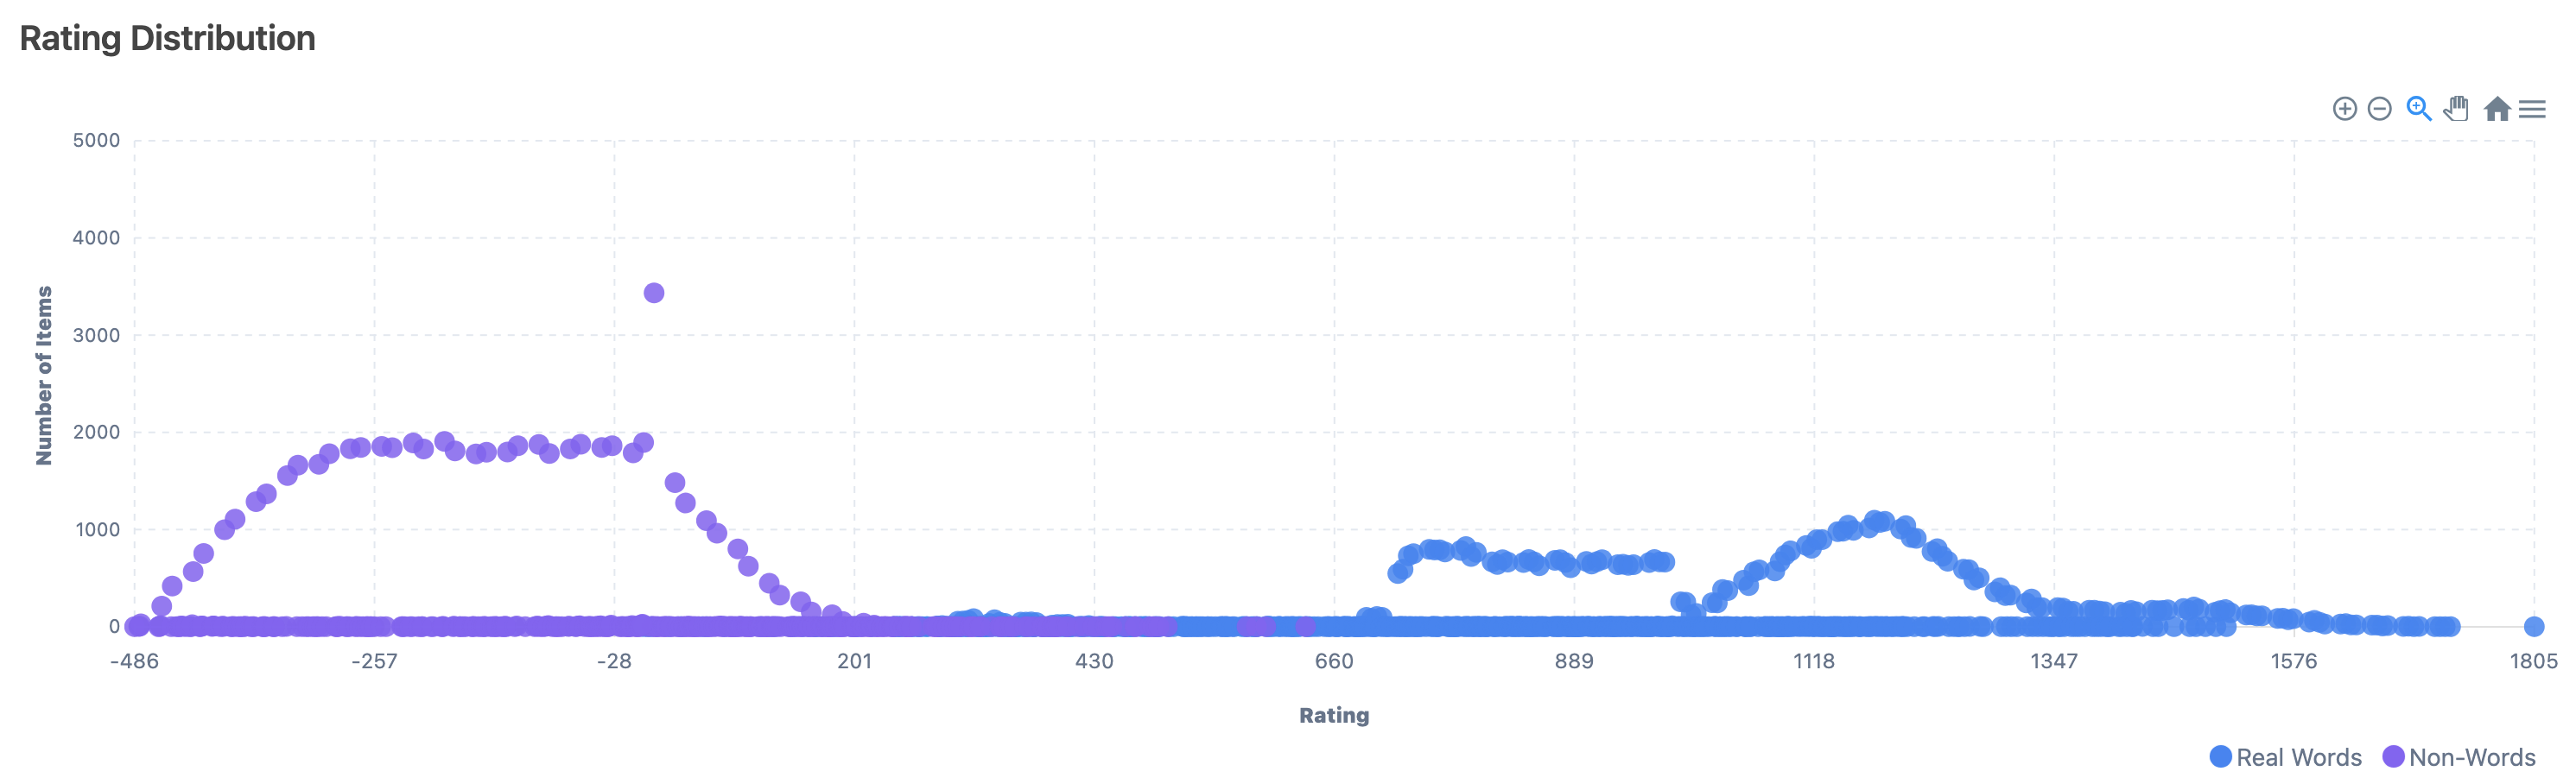
\includegraphics[width=0.9\linewidth]{figures/distribution-items.png}
    \caption{Items distributions after the calibration process is initiated.}
    \label{fig:distribution}
\end{figure}

\subsection{Initialization of the Distractors Rating}
\abbrv{PC}{Proportion of Correct Answers}
The distractors, or pseudo-words being expected to be recognised less frequently, their ratings is expected to go downwards. If the the ratings of the keys (real word types), is capped above zero, in order to show that a test score above zero is symbolically a non-null knowledge of the language, the rating of the distractors can be negative. Otherwise, the distractors would cluster at a rating of zero. For these reason, it was decided to "take advance" on the calibration and give non-words items a random ratings below zero, which means a difference in the average rating between the keys and the distractors. During the selection of the items, this difference is corrected by adding the difference between these means to the rating of the test takers. This has for effect to "punish" more severely the recognition of a non-word that the increase in rating rewarding the recognition a real word. This way, a cheater who consistently pretend to recognize all items (real or not) would face a steep decline in rating, instead of a stable rating.

The figure \ref{fig:distribution} gives a representation of the distribution of the items by ratings. The clusters can be seen hovering over the items which are in the process of being calibrated, which may not number above 10 for a given rating. In a more calibrated distribution, one would see the two line merging in one. As we can see in the same figure, the calibration well advanced for the words of the highest frequency range (the small blue bump below 500 rating), which is exactly the range of test takers for which a simple proportion of correct answer (PC) rating-based test would not be suitable, and for whom a logistic scale such as the Elo rating system is needed.

\section{Items Shortlisting}
From this section onwards, we transition away from the question of the items to focus on the mechanic of the test proper. The test was deployed on a web platform openly accessible without requiring users to create an account\footnote{See \href{https://leksis.bzh}{https://leksis.bzh}}. The behaviours presented in this section happen on the front end of the application. As a test session is expected to use only a small portion of the available items, the idea of shortlisting the available items emerged. Instead of randomly sampling items from the lists of items, which would select almost exclusively items that have not been calibrated, the test select items by unique rating. The items that are not selected during this shortlisting are thus the items clustered at their initial modulo based ratings. Those items would have little chance of being selected without this shortlisting anyway, because in an adaptive setup, they belong in clusters of several hundreds of items. This shortlisting of the available items thus increase the performances for a test session without weighting on the quality of the test. Since the items are shuffled before being selected by unique ratings, the items shortlisted are never exactly the same (especially those which have not been selected yet), thus contributing to the uniqueness of each testing session. In practice, several items with the same rating may still exist after the shortlisting because this selection of item by unique rating is repeated as many times as necessary until the lists of keys and distractors a length of 4000 elements each.

In the case a test taker wants to retake the test after finishing a session, the same (shortlisted) list of items is used, note however that every time an item is selected, it is taken out of the list of available items. This means that someone taking the test a second or third time will never see again the same items. This feature could be used to assess the reliability of the test scores. If the items vary, the only common point between the different testing sessions is the (never fully calibrated) item scores themselves.

\section{The Testing Session}
    \begin{figure}
        \centering
        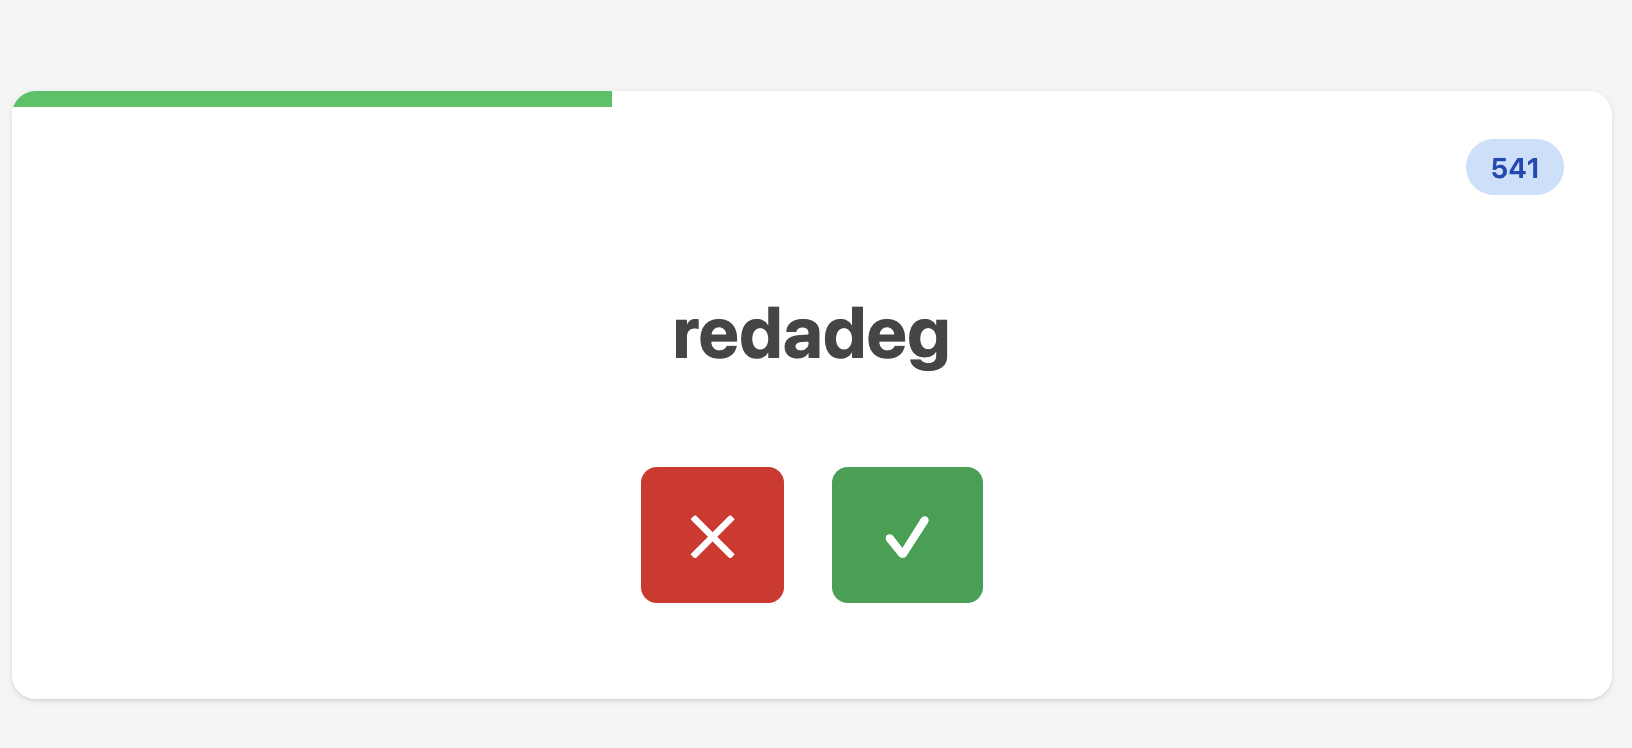
\includegraphics[width=0.5\linewidth]{figures/screenshot-redadeg.png}
        \caption{A screenshot of the test's interface in the middle of Breton language test session.}
        \medskip
        \small
        The word ``redadeg'' is famous in Brittany because of a biannual relay race taking place across the country. Many non-speaker would still recognise this word, which makes the answer from this term a case of the previously mentioned third reason for rating update given for the wrong reason: the rating of the item does not match its real proficiency range. This problem is expected to fade as more people answer the test.
        
    \end{figure}\label{fig:screenshot}

\subsection{User Rating Updates and Session Duration}
The actualisation of the test takers rating takes place in real time and the current rating is shown to them. There are two ways to loose points, by not recognising a real word or by recognising a non-word. Not recognising a non-word does not influence the rating and only recognising real words increases the rating.\\
The logarithmic base for the progression is 10, with a spreading factor of 400, like in chess in order to keep the rating human-readable. The rating is always shown to  It uses the uncertainty function \ref{uncertainty-function}, with $a=100$ and $b=0.5$. This means that a correct recognition of a real word brings 47 points the first time a real word is presented to the test taker, and roughly 8 points after a 100 times, that is, half the result of the uncertainty function because the probabilities of correct answers are always around 50\%. However the uncertainty function is capped to 20 point in order to maintain a steady growth for better performers. The pace of the rating growth is important as the length of a testing session is determined by the current rating, see below the equation that determine the number of real words to be answered.
\begin{equation}
    f(x)=10 + x/14
\end{equation}\label{length-function}
Where $x$ is the current score. This way, a poor performer is not expected to go through a long testing session. Consider a score averaging around 146 (obtained after merely three consecutive good answers), the testing session would only last around 22 items shown (11 real words and around 11 non-words). So ideally, the test would spend three real words to climb up to the test taker's rating, and the 9 remaining items would be used to sort what words do a 150-ish level learner knows and ignores.

When the last real word item is answered, the test results are stored and sent anonymously to the website's data base and the final score is shown to the test taker.

\subsection{Items Selection}
When a test session starts, the program first randomly decides which list it is going to select an item from. If the list selected is the keys, then the items with the closest ratings to the test taker's current rating is selected. As mentioned earlier, when the distractors list is selected, then the difference between the average of the distractors rating and the average of the keys rating is added to the test taker's current rating. If the testee's current rating is 500 and the difference between the average keys and distractors rating is 600, then the test will look for an item with -100 rating. This ensures the diversity of the non-words selected as the test taker's current rating move away from the distractors range.

For performance reasons, the test does not wait an answer to find the next item. It as soon as a new item is displayed on the screen, the test computes the next ratings for the two outcomes, good or bad answers, and selects two items based on these changes in rating. This system, along with the fact that the lists of items are shortened before the start of a session, ensures a smooth and seamless transition after each answer.

\section{Items Rating Update}
The rating of the items is recomputed in the back-end, once a day at midnight, based on the detailed test score stored in the database during the previous day. The system follows the Elo rating system update, also, based on the fact that these updates are asynchronous, one could imagine other systems to update the rating. For example, a real word whose initial rating was 100 not recognised by a test taker whose ultimate score is 500 should probably be increased at least to 500. There must be better ways to update a given item's rating, but ultimately, the time pressure led to a simple update of base on the difference between the prediction and the actual score multiplied by a K-factor of 20 (instead of an uncertainty function). Note however that the expected score of an item is calculated in function of the final score of the test session, not the rating at the moment the item was being answered.

Since the generation of the pseudo-words is expected to produce strings of various degrees of credibility it is admitted that some pseudo-words will be completely unlikely and other pseudo-words will be actual, meaningful words which were never added to a dictionary. This variable credibility would be considered a problem in most applied linguistics experiments, as an equal degree of nonsense is expected from all non-words, but it is an inevitability when items are generated by the tens of thousands. By updating the rating of the non-words, this test instead recognises the fact that all non-words are not created equal, and that unforeseen properties of a pseudo-word may allow people to recognise these strings as actual words. This means that pseudo-words whose rating increases to a point where more than half the test takers would consider it a real word (including more advanced speakers) may eventually be identified and moved from one list to the other. The test does not provide mechanisms to do this yet, apart from downloading the JSON file of the items with their current rating and manipulate the file manually before loading it to the web application again. But the possibility that generated pseudo-words may make sense for test takers is well taken in consideration and the problem is at least partially solved by the current design, as frequently recognised items will deviate from the norm and be shown less and less thank to the update system.

    \section{Adding Languages}
At time of writing, three other languages were added to the platform, Welsh, Ukrainian and French. Base on early test from the Breton test, some changes were made to the procedure of initialising the items ratings. First, the initial ratings for both the keys and the distractors were spread within the same range of ratings, between 0 and 2 000. This was due to the realisation that the large difference in average ratings (between keys and distractors) described above was maybe too large and the degradation in the current rating of the test taker was not reflecting their actual results, as will be explained in the next chapter. The ratings of the distractors were thus evenly spread between 0 and 2 000, while the keys rating were spread between 0 and 1 000 based, in sub-ranges based on frequency lists, while the rest of the keys would be spread randomly between 1 000 and 2 000. The number of items in the 0-1 000 range vary based on the available frequency lists for a given language, but it it understood that only a small portion of the keys would end up in this range. This effectively creates a difference in average ratings between the keys and the distractors, albeit a more reasonable one. Details of the code use for each specific language can again be found on GitHub\footnote{Find the specifics for a given language by their IETF language code in \href{https://github.com/Oktogazh/sudogen/tree/master/locales}{this directory}, with the file 4.ipynb being the one responsible for the initialization of the items ratings.}

    \section{Feedback}
\abbrv{LLM}{Large Language Model}
Since a widespread use of the test is essential to better calibrate the items ratings, two strategies were developed to increase engagement. First, the ability for users to share their scores with a link to the test. Second, an elaborated large language model (LLM) prompt that integrates the results of the test, destined to build a constructive feedback by teaching the meaning of the unrecognised words. This personalised and interactive lesson focuses on the words with the lowest rating, then asking the user to build sentences using the new words. After which it proposes to go deeper in elaborating on these word, by showing multimedia content that use the words words, or to keep going in learning about the other unrecognised real words. The prompt can be copied and pasted to the user's favourite LLM, or, if the navigator allows it, directly shared with the LLM app with the \href{https://developer.mozilla.org/en-US/docs/Web/API/Navigator/share}{navigator.share()} API. The version of the prompt at time of writing can be found in Appendice \ref{chp:Analysis Prompt}, along with an example of answer from GPT-5.

\begin{figure}[htbp]
    \centering
    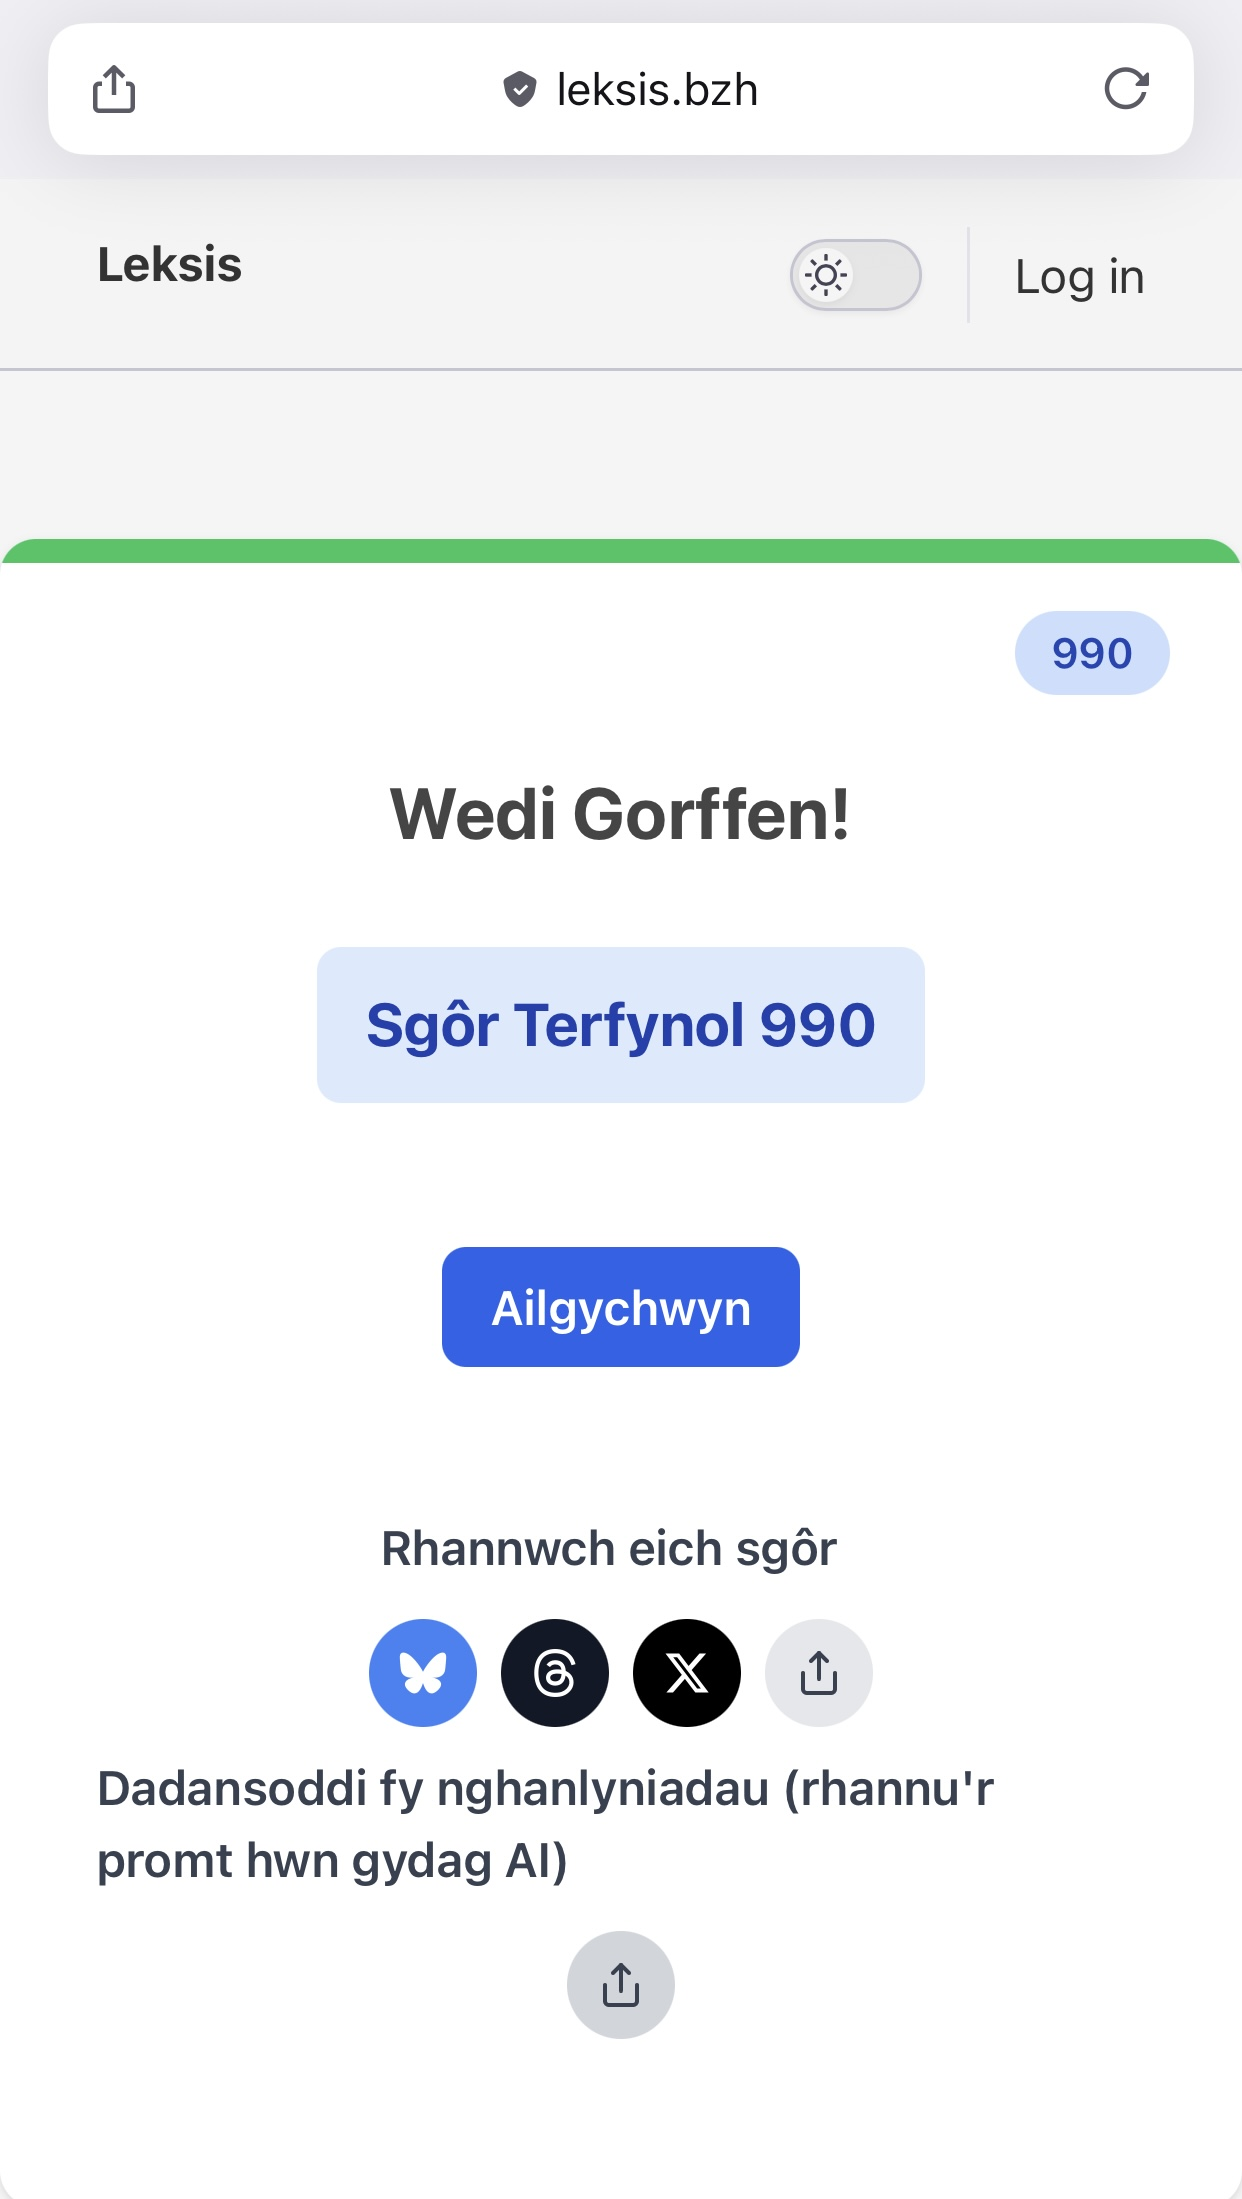
\includegraphics[height=0.7\textwidth]{figures/end-screen.jpg}
    \caption{End screen with the score, share link and analyse prompt button}
\end{figure}\label{fig:endscreen}

\section{Validation}
\subsection{Construct Validity and Design Choices}
In the domain of psychometrics, when the traits measured are latent, it is essential to test the tests, a process called validation. Validation theory is dominated by principles established by \textcite{messick_validity_1987} who unified different aspects of validity, thus simplifying previous approach to the matter.\ \textcite{borsboom_concept_2004} on his end, attempted to simplify construct validity discution a step further by incisting on key concepts in the scientific method, ontology, meaning, causation. Borboom pointed out that much of the construct validity discussion was more about the validation processes than the validity of the constructs themselves. His argument was, consciously or not, integrated in~\cite{kane_validating_2013}. This paper introduced an argument-based approach to validation, where a given test must be proposed along a set of claims, which must be tested individually.

As far as construct validty is concerned, the first half of the literature review showed how a LDT vocabulary test can be used to indirectly measure other constrcuts of proficiency. The concern of this dissertation is not the validation of the construct itself, but the validation of the calibration methodology and the scoring system. This includes the following:

\begin{enumerate}
  \item The use of a logarithmic scale as a knowledge model, to represent the difficulty rating of the items.
  \item The use of frequency lists for the ratings initialisation.
  \item The use of the ``beans'' modulo clustering technique to increase the chances of encountering better calibrated items and optain meaningfull results without a full calibration.
\end{enumerate}

The first point, the use of a logarithmic scale, by its statistical nature, is valid. At least in a context where a large enough number of tests are taken to calibrate the items. The real issue with the current framework is its ability work without an extensive calibration. This is why the focus of the validation process must be on the two other design choices. To validate these design choices, we must make inferences on how the test would behave under certain condition. To make sure that the test would capture small variation in vocabulary level, these two inferences must be verified:

\begin{enumerate}
  \item \textbf{Reliability}: People taking the test several times in a row will obtain a similar score. Below 1000, the items initial rating are random values within some range. In French the 1000 most frequent items are randomly rated between 0–400, the 1000 to 2000 most frequent words between 400–500 and so on. By ``similar'' we mean that the scores stay within such a range.
  \item \textbf{No ceiling effects}: People with different vocabulary level should not get stuck in the same score range. Three critical ranges can be identified: around 0, where beginer would end up with a null score despite some vocabulary knowledge; aroud 1000, where the ratings cease to be defined based on frequency and start to become truly random; around 2000, where all fluent speakers would know enough words to have a positive ratio along the 1000–2000 range.
\end{enumerate}

The most complete way to verify these inferences would be to run an integration test. Take a group of beginners in a year-long intensive course for adults and collect the results at taking the test every single week. Inspect how fast the students progress, where they stagnate, be it at similar periods in time (around holidays) or at similar score level, which would indicate a ceiling effect.

Such an integration test cannot be made in the span of time covered by a dissertation. But the early development of tests for a few language may still bring insights on the matter. Especially regarding reliability, it is possible to inspect anonymous test results to see how stable the predictions become as a test session is carried on. If the score is accurate, the chance of recognising real words are around 50\%, which is a falsifiable claim. However, validating the reliability of the test does not inform on the potential ceiling effect.

\subsection{Clarifications and Results Interpretation}
Before ending this chapter, we want to clarify a few points in order avoid a misinterpretation of the results. Especially, it is understood that a growth in the test-taking skill should not be generalized blindly. That it can interpreted as proficiency growth only as long as the learning activity consist of a real use of the language, where the vocabulary is learned within the use of grammatically correct sentences. Taking the test repeatedly may make the test taker being better at taking the test without improving their proficiency proper. Finally, it is understood that tests score cannot be universally interpreted in a similar way, 1500 in the Welsh test and the French test cannot be worth the same thing for the following reasons:
\begin{enumerate}
  \item Socio-linguistic differences make it difficult to find equivalence in the idea of fluency.
  \item The number of items is different for different languages, the initialisation of the items rating is based on frequency lists of different lengths. This leads to different scores at equivalent vocabulary sizes.
  \item Considering that a wide-spread usage of the tests change the ratings dramatically, the rating of the items will have a tendency to cluster around the level of the test takers demographics. If many very fluent people take one test, the ratings value will be devaluated. If many beginners take a test, the items rating will be subject to an inflationary effect.
\end{enumerate}

None of the aspects cited above are seen as a problem for the intended goal of the test. The test aims at measuring the dynamics, the speed at which the learners acquire language over periods of weeks and months. For this purpose only reliability and the absence of ceiling effects are needed.
